\documentclass[conference]{IEEEtran}
\IEEEoverridecommandlockouts

\usepackage[utf8]{inputenc}
\usepackage[lithuanian]{babel}
\usepackage[T1]{fontenc}


% The preceding line is only needed to identify funding in the first footnote. If that is unneeded, please comment it out.
\usepackage{cite}
\usepackage{amsmath,amssymb,amsfonts}
\usepackage{algorithmic}
\usepackage{graphicx}
\usepackage{textcomp}
\usepackage{xcolor}
\def\BibTeX{{\rm B\kern-.05em{\sc i\kern-.025em b}\kern-.08em
    T\kern-.1667em\lower.7ex\hbox{E}\kern-.125emX}}

\usepackage[labelsep=endash]{caption}
\renewcommand{\figurename}{pav}
\renewcommand\IEEEkeywordsname{Raktažodžiai}

\usepackage{lipsum}  




\begin{document}

\title{Matematikos Sprendimas}

\author{\IEEEauthorblockN{Dominykas Dulevičius}
\IEEEauthorblockA{\textit{Informatikos institutas} \\
\textit{Matematikos ir informatikos fakultetas}\\
Vilnius, Lietuva \\
dominykas.dulevicius@mif.stud.vu.lt}
\and
\IEEEauthorblockN{Arnas Bulka}
\IEEEauthorblockA{\textit{Informatikos institutas} \\
\textit{Matematikos ir informatikos fakultetas}\\
Vilnius, Lietuva \\
arnas.bulka@mif.stud.vu.lt}
\and
\IEEEauthorblockN{Pijus Kizerskis}
\IEEEauthorblockA{\textit{Informatikos institutas} \\
\textit{Matematikos ir informatikos fakultetas}\\
Vilnius, Lietuva \\
pijus.kizerskis@mif.stud.vu.lt}
}

\maketitle

\begin{abstract}
Projektinio darbo metu tyrėme ir lyginome internete paplitusių populiarių modelių
galimybes ir tikslumą sprendžiant matematinius uždavinius bei lyginome rezultatus su
TP-Transformer tipo modeliu, kuris buvo specialiai aptreniruotas su DeepMind kūrėjų
„Mathematics-Dataset“ duomenų rinkiniu.
\end{abstract}

\begin{IEEEkeywords}
TP - Tenzoriaus-Produkto
\end{IEEEkeywords}

\section{Įvadas}
Pristatote problemą

\section{Duomenų Rinkinys}

\subsection{Metodas A}

Pristatote naudojamus metodus

\begin{equation}
\mathcal{L}({\bf X}, {\bf Y}) = \frac{1}{w \cdot h} \sum_{i=1}^h \sum_{j=1}^w (X_{i, j} - Y_{i, j})^2
% \label{eq:lygtis1}
\end{equation}

% Taikyta nuostolių funkcija ~\eqref{eq:lygtis1}.

\begin{align}
y & = f(x) \nonumber \\
f & = f_1(f_2(x))
% \label{eq:lygtis2}
\end{align}

% Taikytas modelis ~\eqref{eq:lygtis2}.


\section{transformer}

\subsection{Veikimas}
Populiariausias bei plačiausiai paplitęs natūralios kalbos modelis - transformeris. Jis pakeitė LSTM (angl. \textit{Long Short-Term Memory}) aplenkdamas pastarajį tiek efektyvesniu apmokymu, tiek tikslesniais bei greitesniais atsakymais. LSTM modelis tekstą apdoroja eidamas per kiekvieną žodį iš eilės bandydamas "prisiminti" visą sakinio esmę. Transformeris apdoroja kiek įmanoma daugiau teksto vienu metu ir, atkreipdamas dėmesį į raktinius žodžius bando suprasti teksto esmę.

\centerline{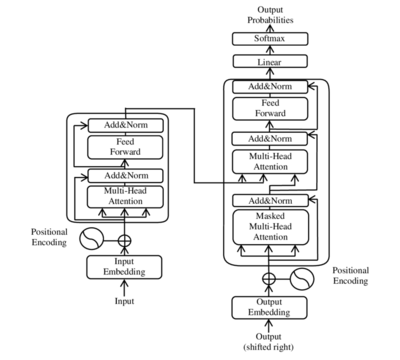
\includegraphics{transformer.png}}

\subsection{Moduliai}
Iš pirmo žvilgsnio modelio architektūra gali pasirodyti sudėtinga (1 pav.?), tačiau ją galima išskirti į dvi pagrindines dalis:
\begin{itemize}
  \item \textbf{Koduotuvas} (angl. \textit{Encoder}) yra atsakingas už įeities duomenų susistemizavimą bei užkodavimą. Tai modeliui padeda suvienodinti gaunamus duomenis bei juos paruošti kitam transformerio moduliui - dekoderiui.
  \item \textbf{Dekoderis} (angl. \textit{Decoder}) iš koduotuvo gauna galutinę paslėptą būseną pagal kurią sprendžia kiekvieno žodžio svarbumą. Susidėliojęs konteksto vektorių dekoderis atiduoda galutinę išvestį.
\end{itemize}
\subsection{Dėmesys}
Turbūt svarbiausias transformeryje naudojamas sluoksnis - susifokusavimas (angl. \textit{self-attention}). Būtent dėl šios savybės transfomeris geriau gali perprasti tekstą. Susifokusavimas figūruoja tiek koduotuvo, tiek dekoderio moduliuose padėdamas išgauti "paslėptas" būsenas bei apskaičiuoti kiekvieno įvesto žodžio svarbumą. 

\subsection{Equations}



\subsection{Paveikslėliai ir lentelės}

% Paveikslėlį cituojame ``~\ref{fig} pav.''.

% Paveikslėlį cituojame ``~\ref{tab1} lentelė''.

\begin{table}[htbp]
\caption{Lentelės aprašas}
\begin{center}
\begin{tabular}{|c|c|c|c|}
\hline
a & b & c &  d \\
\hline
\end{tabular}
\label{tab1}
\end{center}
\end{table}

% \begin{figure}[!h] % įterpti čia
% \centerline{
\includegraphics{fig1.png}}
% \caption{Paveikslėlio aprašas.}
% \label{fig}
% \end{figure}


\section{Naudojami Apmokyti Modeliai}
Lyginti su TP-Transformer pasirinkome 5 iš anksto apmokytus klausimų-atsakymų modelius: \textbf{
iAsk.Ai, DeepAI, Bing AI}, .... Šių modelių tikslumą matematikos uždavinių sprendimui lyginsime su \textbf{ischlag/TP-Transformer} modeliu,
specialiai pritaikytų matematikos uždaviniams spręsti.

\subsection{ischlag/TP-Transformer}
Šio modelio sukūrimui į standartinį transformerio tipo modelį buvo integruota Tenzoriaus-Produkto
reprezentacija, tokiu būdu pagerinant išskirtinius sąryšius tarp transformerio vidinių struktūrų. Modelis buvo apmokytas
naudojant „Mathematics-Dataset“, kuris buvo išskaidytas į 56 skirtingas matematikos šakas, siekiant
pagerinti modelio tikslumą bei atpažinamumą. Mūsų pasirinkta iš anksto ištreniruota modelio 
versija buvo treniruojama su 1.7 milijono duomenų.

\subsection{iAsk.Ai}
Šis kalbos variklis naudoja panašias technologijas, kaip ir \textbf{ChatGPT} variklis, tačiau
papildomas dėmesys yra skiriamas optimizuoti natūralios kalbos aprodorojimo modelį. iAsk AI taip pat susideda iš specialiai pritaikyto,
didelio masto Transformerio kalbos modelio. Šis modelis buvo išskirtinai mokomas remiantis
patikimiausiais ir autoritetiškiausiais literatūros bei interneto šaltiniais,
kas suteikia iAsk AI galimybę atsakyti į klausimus objektyviai,
faktiškai ir be potencialaus subjektyvumo, kurio galėtų būti ChatGPT.

\subsection{Bing AI}
BingAI - Microsoft kompanijos sukurtas dirbtinio intelekto variklis, naudojamas Bing paieškos sistemoje. Šis variklis naudoja tokias technologijas kaip gilųjį, mašininį mokymą ir natūralios kalbos apdorojimą, siekiant pagerinti paieškos rezultatus ir suteikti geriausius atsakymus vartotojams. Bing AI - nuolat tobulinamas ir mokomas naujų uždavinių, kad būtų užtikrinta patikima ir tiksli paieška. Taip pat Bing AI taikoma kitose Microsoft produktuose, tokiuose kaip Cortana ir Microsoft 365.

\subsection{DeepAI}
DeepAI - GPT-2 modeliu paremtas natūralios kalbos modelis. Šio, kaip ir kitų kalbos modelių, architektūroje slepiasi su dideliu kiekiu duomenų apmokytas transformeris.
\section{Tyrimo Eiga}
Iš „Mathematics-Dataset“ duomenų rinkinio 56 matematinių uždavinių kategorijų išsirinkome
po dvi klausimų-atsakymų poras. Iš viso gavosi duomenų rinkinys, su 112 klausimų ir 112 atsakymų.
Tada visus klausimus uždavėme 5 pasirinktiems klausimų-atsakymų modeliams bei ischlag/TP-Transformer modeliui ir skaičiavome
tikslumą - kiek iš užduotų klausimų modeliai sugebėjo atsakyti teisingai.
Klausimų ir atsakymų pavyzdžiai iš kiekvienos temos:
\subsection{Algebra}
\begin{itemize}
    \item Klausimas: Suppose -2*i + 20 = 5*o, 2*o - 4 = 3*i + o. Suppose -g + 2 = i, 4*g - 6*g = -5*u - 19. Let f be -6 + 3 + 2 + u/(-1). Solve -f*l = -l for l.
    \item Atsakymas: 0
\end{itemize}
\subsection{Aritmetika}
\begin{itemize}
    \item Klausimas: What is the tenth root of 95210445 to the nearest integer?
    \item Atsakymas: 6
\end{itemize}
\subsection{Matematinė Analizė}
\begin{itemize}
    \item Klausimas: Let s(w) be the third derivative of -7*w**2 - 1/30*w**5 - 23/6*w**3 + 0 + 0*w**6 + w - 1/42*w**7 + 1/24*w**4. What is the second derivative of s(l) wrt l?
    \item Atsakymas: -60*l**2 - 4
\end{itemize}
\subsection{Palyginimas}
\begin{itemize}
    \item Klausimas: Suppose -15*p + 48 + 27 = 0. Suppose 13 = 5*f - p*n - 2, 0 = 3*f - 2*n - 8. Let d be (-3 + 110/36)*f. Which is the third biggest value?  (a) 1/6  (b) d  (c) -4
    \item Atsakymas: c
\end{itemize}
\subsection{Konvertavimas}
\begin{itemize}
    \item Klausimas: How many micrometers are there in seven halves of a millimeter?
    \item Atsakymas: 3500
\end{itemize}
\subsection{Skaičių Operacijos}
\begin{itemize}
    \item Klausimas: Let a(s) = -154*s + 138. Let x be a(0). Let r(f) = -f - 3. Let z be r(-5). Suppose 4*v + u + u - 282 = 0, -2*v + z*u = -x. What are the prime factors of v?
    \item Atsakymas: 2, 5, 7
\end{itemize}
\subsection{Daugianariai}
\begin{itemize}
    \item Klausimas: Simplify ((y/y**(1/4)*y)**(3/47)*(y*y*y*y**(4/7)*y*y)/y**5)/(y/((y/(y*y/y**(-2/3)))/y*y*y)*(y*y/(y/(y**2/y)))/y*y**7/y**(4/3)) assuming y is positive.
    \item Atsakymas: y**(-30203/3948)
\end{itemize}
\subsection{Tikimybės}
\begin{itemize}
    \item Klausimas: Four letters picked without replacement from {a: 1, b: 1, s: 1, r: 1, q: 2, f: 2}. Give prob of sequence rbaq.
    \item Atsakymas: 1/840
\end{itemize}

Modelio spėjimai bus klasifikuojami kaip binariainiai: arba modelis atspėjo atsakymą, arba ne.
Atsakymas bus laikomas teisingu tik tuo atveju, jei buvo grąžintas lygiai toks pat, kaip ir buvo tikimasi atsakyme.
Kaip vienas iš pavyzdžių galėtų būti: jeigu tikėtas atsakymas buvo sveikasis skaičius, bet modelis grąžino
nesupaprastintą trupmeną, nors rezultatas yra toks pat, atsakymas buvo užskaitytas kaip neteisingas.
Tikslumo metrika bus skaičiuojama padalinant teisingai atspėtų klausimų skaičių iš visų klausimų skaičiaus.

\section{Rezultatai}

\section{Išvados}


% Cituojame šaltinį \cite{lecun2015deep}.

\bibliographystyle{plain}
\bibliography{saltiniai}

\end{document}
